% !TeX program = xelatex
\documentclass[11pt]{ctexart}
\usepackage[margin=1in]{geometry}
\usepackage{amsmath,amssymb,booktabs,graphicx,microtype,xcolor}
\usepackage[colorlinks=true,linkcolor=blue,urlcolor=blue,citecolor=blue]{hyperref}

\newcommand{\todo}[1]{\textcolor{red}{[待补：#1]}}
\newcommand{\cmh}{CMH}
\newcommand{\swa}{\mathrm{SWA}}

\title{\textbf{蒸馏门控联想记忆：\\一种具有固定状态全局通道的滑窗混合语言模型}\\[0.6em]
\large Yile Ma\\[0.2em]
\normalsize 2026 年 11 月}
\date{}

\begin{document}
\maketitle

\begin{abstract}
注意力机制是 Transformer 语言模型的主要计算开销，训练时随序列长度二次增长。线性注意力与状态空间模型消除了这一开销，但在需要\textbf{精确取回早前 token} 的任务上系统性地弱于全注意力。本文研究知识蒸馏能否修复这一权衡。我们提出 \cmh{}（Compressed-Memory Hybrid，压缩记忆混合架构）：一种双通道块，用滑窗注意力处理局部交互，用\textbf{门控联想记忆}处理全局上下文——即一个固定大小的外积键值状态，配有 (i) 逐 token 显著性写入门控（决定"什么值得记"）与 (ii) 逐头可学习保留率（决定"记多久"）。

我们首先给出一个受控的\textbf{负结果}：在 2--40M 参数规模下从零训练的 \cmh{} 继承了线性注意力家族的检索弱点——成本曲线与全注意力持平（吞吐至 4096 token 保持平坦、峰值显存节省 78\%），但无法学会精确长程召回。通过六轮受控设计迭代（softmax 记忆槽、sigmoid 门控槽、课程学习、扩大状态），我们将根因定位为\textbf{软检索冷启动}问题：精确寻址要求位置嵌入先学出近正交的对齐几何，读分布才能被梯度锐化，而从零训练可获得的稀疏任务信号无法引导出这一几何。

随后我们检验了 token 级蒸馏能否拯救记忆通道。结论是：不能。来自 GPT-2 的蒸馏使 38M 参数的 \cmh{} 学生停留在 5.40 nats（从零训练为 5.44）；来自\textbf{域内}全注意力教师——其在本文语料上比 GPT-2 好 0.7 nats——的蒸馏同样无效（5.56）。与此同时，纯滑窗消融在 TinyStories、序列长度 512 上与全注意力持平（1.79 对 1.80），说明该语料几乎不需要全局上下文——而 \cmh{} 的固定状态通道相对它所增强的纯滑窗模型\textbf{净损失 3.65 nats}。我们的结论是：在 $\le$40M 规模下，固定状态全局通道的质量差距是\textbf{架构性的}而非优化假象——无论教师强弱，稠密监督都无法弥合其中的任何部分。效率优势是真实的，但在检索冷启动被架构手段解决之前（delta-rule 写入、硬寻址），保留全注意力层的混合设计依然是合理的。全部训练日志、消融与分析代码随文公开。
\end{abstract}

\section{引言}\label{sec:intro}

Transformer 语言模型的计算开销由注意力主导：训练时随序列长度二次增长，生成时正比于 KV 缓存长度。十余年的架构研究——线性注意力 \cite{katharopoulos2020}、门控变体 \cite{yang2023gla,peng2023rwkv}、状态空间模型 \cite{gu2023mamba}、滑窗注意力 \cite{beltagy2020longformer}——产出了单 token 成本恒定的高效替代品。然而一条一致的经验规律浮现出来：在需要\textbf{精确检索}的任务（长距离复制、计数、查找）上，这些模型落后于全注意力 \cite{waleffe2024jamba}。

工业界的对策是混合化：在大量高效层之间保留少量全注意力层（Jamba \cite{waleffe2024jamba}、Zamba \cite{glorioso2024zamba}、Hymba \cite{wang2024hymba}）。全注意力层充当线性层学不到的精确检索能力的"兜底"。本文研究一个不同的问题：

\begin{quote}\itshape
兜底层能否被"来自预训练教师的知识蒸馏"取代——从而让\textbf{整个}网络都是高效的，而不是其中一部分？
\end{quote}

回答这个问题需要一个值得修复的全局通道架构，以及对"从零训练为何失败"的精确理解。本文贡献：

\begin{enumerate}
\item \textbf{\cmh{} 块}（\S\ref{sec:method}）：双通道设计，其全局通道以两个显式机制区别于已有线性注意力状态——\textbf{逐 token 写入门控} $g_t=\sigma(W_g x_t)$（让模型自己决定什么值得记）与\textbf{逐头可学习保留率} $\gamma_h=\sigma(\theta_h)$（让不同的头自主学习记多久）。
\item \textbf{受控失败分析}（\S\ref{sec:scratch}）：六轮设计迭代，在带全注意力与纯滑窗对照的召回诊断任务上，系统比较记忆槽、sigmoid 门控、外积联想记忆、课程学习与扩大状态。我们将失败定位为软检索冷启动并给出机制解释。据我们所知，此前没有工作以这种架构控制力度隔离过该现象。
\item \textbf{蒸馏无法拯救记忆通道}（\S\ref{sec:exp}）：来自弱域外教师（GPT-2）与强域内全注意力教师的 token 级 KL 蒸馏，都使 \cmh{} 停留在约 5.5 nats——相对其自身的纯滑窗消融差 3.65 nats——证明差距是架构性的，而非优化信号问题。
\item \textbf{效率画像}（\S\ref{sec:efficiency}）：固定状态设计使吞吐从 256 到 4096 token 保持平坦（4096 时为全注意力的 15.2 倍），峰值显存节省 78\%。
\end{enumerate}

\section{相关工作}\label{sec:related}

\textbf{高效注意力。}线性 Transformer \cite{katharopoulos2020} 用核化形式取代 softmax 注意力，其键值状态是固定的外积矩阵；GLA \cite{yang2023gla} 与 RetNet \cite{sun2023retnet} 加入门控与衰减；RWKV \cite{peng2023rwkv} 与 Mamba \cite{gu2023mamba} 转向递归与选择性状态空间。它们共有的、与本文分析相关的性质是：读取是已存键值绑定的（归一化）求和，因此精确检索要求写入的键近乎正交——这是\textbf{涌现性质而非架构保证}。

\textbf{混合架构。}Jamba \cite{waleffe2024jamba}、Zamba \cite{glorioso2024zamba}、Samba \cite{wang2024samba}、Hymba \cite{wang2024hymba} 在高效块之间交错少量全注意力层，并一致报告全注意力层对检索密集评测不可或缺。本文由同一观察出发，但用训练信号工程（蒸馏）而非架构混合来应对。

\textbf{跨架构蒸馏。}MOHAWK \cite{wang2024mohawk} 与 Mamba-in-Llama \cite{wang2024mambaillama} 将 Transformer 教师逐层蒸馏进 Mamba 式学生，把注意力结构转移为递归状态；Hinton 式 logit 蒸馏 \cite{hinton2015distill} 提供我们所用的稠密监督信号。相对于这些工作，本文的差异是 (i) 不同的学生架构——带显式显著性门控与逐头保留率的双通道设计；(ii) 对冷启动现象的显式前后对照研究——这正是整个方法的动机。

\textbf{小模型试验场。}TinyStories \cite{eldan2023tinystories} 证明了连贯语言能力可在精选语料上于 1--33M 规模涌现，使其成为本文规模下架构比较的标准试验场。

\section{方法：\cmh{} 块}\label{sec:method}

\subsection{结构}

序列按块大小 $w$ 分块：\textbf{块内并行、块间串行}，因此块天然因果。每层维护状态
\[
S \in \mathbb{R}^{h \times d_h \times d_h}, \qquad n \in \mathbb{R}^{h \times d_h},
\qquad d_h = d/h,
\]
在每个序列开始时初始化为零。对每个块内的每个 token $x_t$，依次执行四步。

\textbf{(1) 联想读取。}状态只含之前所有块的信息；读取是对已存绑定的归一化检索：
\begin{equation}
o_t \;=\; \frac{q_t^{\top} S}{q_t^{\top} n + \epsilon}, \qquad q_t = W_r x_t .
\label{eq:read}
\end{equation}
除以 $q_t^\top n$ 使读取成为已存值的凸组合，类似均值聚合检索；$n$ 累积（门控后的）键，使读取能适应每个键方向已接收的质量。

\textbf{(2) 滑窗注意力（局部通道）。}读取残差接入后，施加因果滑窗注意力（窗口 $w$、attend-only 上下文 $w$，即前一块作为上下文；步长 $w$、有效跨度 $2w$）：
\begin{equation}
\tilde{x}_t \;=\; x_t + W_o o_t \;+\; \swa(x)_t .
\end{equation}

\textbf{(3) FFN。}标准 MLP，扩展系数 4，GELU 激活。

\textbf{(4) 门控联想写入。}块输出以逐 token 显著性门与逐头衰减写入状态：
\begin{align}
S &\leftarrow \gamma \odot S + (g_t\, k_t)^{\top} v_t,
& k_t &= W_k \tilde{x}_t, \quad v_t = W_v \tilde{x}_t, \\
n &\leftarrow \gamma \odot n + \textstyle\sum_t g_t\, k_t, &
g_t &= \sigma(W_g \tilde{x}_t), \quad \gamma_h = \sigma(\theta_h),
\end{align}
其中 $\theta_h$ 逐头可学习（初始化为 3.0，即每块保留率 $\gamma\approx 0.95$）。

\subsection{推导}\label{sec:derivations}

\textbf{读取即凸组合。}设已存（门控后）键值对为 $\{k_i\}, \{v_i\}$，则
$S = \sum_i k_i v_i^{\top}$、$n = \sum_i k_i$。对 $q_t^{\top} n > 0$ 的查询，式~\eqref{eq:read} 展开为
\begin{equation}
o_t \;=\; \frac{\sum_i (q_t^{\top} k_i)\, v_i}{\sum_i (q_t^{\top} k_i)}
\;=\; \sum_i \alpha_i\, v_i, \qquad \alpha_i \;=\; \frac{q_t^{\top} k_i}{\sum_j q_t^{\top} k_j},
\label{eq:convex}
\end{equation}
即以\textbf{线性（未指数化）权重} $\alpha_i$ 对已存值做凸组合。两个推论：其一，检索质量受键几何约束——要精确恢复某个 $v_j$，需要 $q_t^{\top} k_j$ 远大于其余所有 $q_t^{\top} k_i$，即键集合在 $d_h$ 维空间中近似正交。$d_h=32$ 的诊断规模下每头最多能同时区分约 $d_h$ 个键；单头变体（$d_h{=}128$）把上限放宽到约 128——这正好解释了 \S\ref{sec:scratch} 中它改善窗口外召回的原因。其二，softmax 注意力计算的是同一种混合，但权重经过指数化：$e^{q_t^{\top} k_i / \sqrt{d}}/Z$，有效锐度随键--查询对齐程度\textbf{乘性}增长，而式~\eqref{eq:convex} 只\textbf{线性}增长。这是 \S\ref{sec:scratch} 冷启动论证的数学内核：几何未对齐时，softmax 仍能锐化最优匹配，线性混合无法放大相对差异。

\textbf{状态容量对 KV 缓存。}每层状态持存 $h \cdot d_h^2 + h \cdot d_h$ 个数——学生规模下 $4 \times 32 \times 32 = 4{,}096$ 加 128——与上下文长度无关。全注意力的 KV 缓存在 $N$ 个 token 后持存 $N \cdot d$ 个数（教师 124M、$N{=}512$、$d{=}768$ 时为 393{,}216）。压缩比按设计随长度变化。复制诊断要求 4{,}096 个状态数足以容纳 64 个 $d_h$ 维绑定并保持线性读取可分辨的间距。gap${\ge}192$ 的失败与上文的几何约束一致而非与原始容量矛盾：单头变体的 $128{\times}128$ 状态容纳 64 个绑定绰绰有余，但填充 token 进入同一键空间后召回仍然坍塌。

\textbf{成本核算。}每层每 token：窗口通道 $O(w \cdot d)$ MAC（分数与值各一次），记忆通道读写各 $O(d_h^2)$，FFN $O(4d^2)$。学生配置合计约 0.75M MACs/token/层，全注意力在 $N{=}512$ 时约 1.3M——且后者随 $N$ 线性增长，\cmh{} 恒定。\S\ref{sec:efficiency} 的实测吞吐交叉点与此核算吻合。

\begin{figure}[t]
\centering
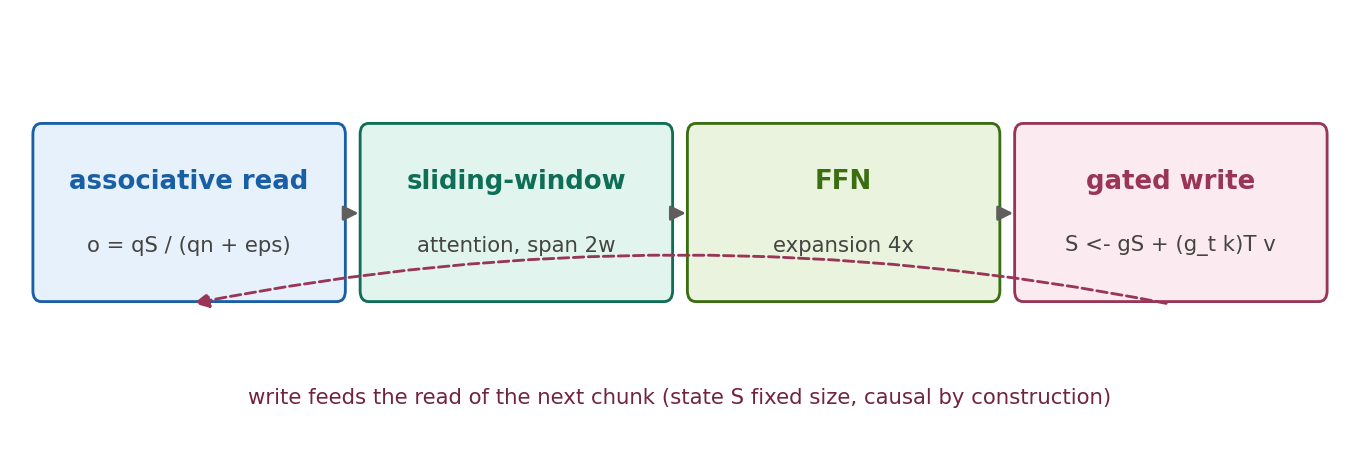
\includegraphics[width=0.95\textwidth]{fig_arch.png}
\caption{一个 \cmh{} 块。序列按 $w$ token 分块；虚线箭头是跨块递归——固定大小的状态 $S$ 从写入流向下一块的读取。块内注意力在其窗口上因果；前一块作为 attend-only 上下文。}
\label{fig:arch}
\end{figure}

\subsection{设计依据：为什么是外积记忆}

我们的早期设计使用固定数量 $M$ 的\textbf{显式记忆槽}：每个槽累积被分配到它的值——分配方式或为对 token 的 softmax 分配，或为 sigmoid 门控。两者在长程召回上全部失败（\S\ref{sec:scratch}）。机制原因：槽的\textbf{地址}（读取所用的键）由槽内累积值派生，且槽分配会冲淡任何单个 token 的贡献——64 个前缀 token 被 384 个共享相同键质量的填充 token 稀释。而外积形式中，\textbf{每个写入的 token 都贡献一个带自己键的绑定 $(k_t, v_t)$}，按内容或位置对齐的检索从架构上就是可表示的。这一区别被 \S\ref{sec:scratch} 的实验直接证实。

\subsection{工程细节}

训练使用 bf16 自动混合精度 + fp32 主权重、微批梯度累积（每微步 8 条 512 token 序列）、梯度裁剪 1.0、AdamW（$\beta_1{=}0.9$，$\beta_2{=}0.95$，权重衰减 0.1）。原型的 Python 分块循环未做优化；融合核（块对角注意力 + 批量状态更新）可进一步提升绝对吞吐，但不影响扩展性结论。

\section{为什么从零训练会失败}\label{sec:scratch}

\subsection{诊断任务}

用\textbf{复制}任务探测精确长程召回：输入 = $L{=}64$ 个随机 token（前缀）+ gap 个填充符 + 回声段（须复述前缀）。回声位置 $j$ 的预测需要跨越 $(L+\mathrm{gap})$ 的距离取回前缀 token $j$。有效窗口 $2w=256$ 时，gap 超过约 192 后记忆通道是唯一通路。所有模型为因果语言模型，训练 3--8k 步、batch 16，回声位置交叉熵加权 $8\times$；准确率在 64 个回声预测上度量。

\subsection{六轮受控迭代}

所有轮次使用相同骨架（诊断规模 8 层、$d{=}128$），只改全局通道：

\begin{table}[h]
\centering
\caption{复制诊断上的设计迭代。gap=32 在窗口内；gap$\ge$192 需要记忆。所有轮次中全注意力在 gap=384 达到 1.00，纯滑窗 0.23。}
\label{tab:iterations}
\begin{tabular}{llll}
\toprule
迭代 & 全局通道 & gap=32 & gap$\ge$192 \\
\midrule
1 & softmax 记忆槽（$M{=}32/64/128$） & 0.03 & $\approx$ 随机 \\
2 & + sigmoid 槽门控、锐化读取 & 0.03 & $\approx$ 随机 \\
3 & 外积联想记忆 & \textbf{0.69} & 0.03--0.15 \\
4 & + gap 课程学习（32$\to$384） & 0.07 & 0.14 \\
5 & 单头大状态（$128{\times}128$） & --- & 0.16（gap 256）、0.25（gap 320） \\
6 & 真滑窗（修复块注意力 bug） & \textbf{0.69} & 不变 \\
\bottomrule
\end{tabular}
\end{table}

\begin{figure}[t]
\centering
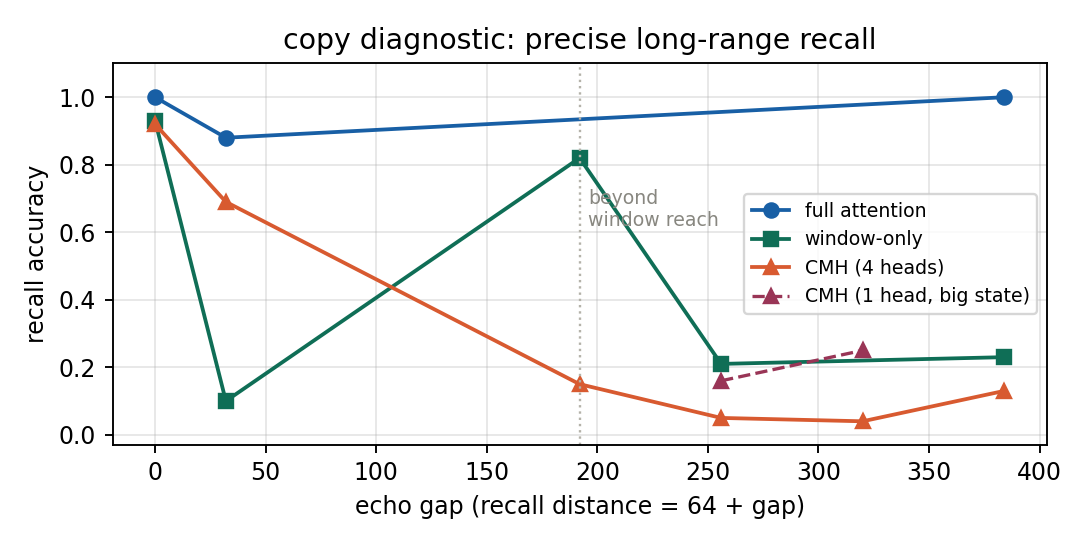
\includegraphics[width=0.95\textwidth]{fig_gapsweep.png}
\caption{复制诊断的召回准确率随回声间隔的变化。竖虚线标记前缀超出 256 有效窗口的位置，只有记忆通道能跨越它。单头变体（虚线）把每头状态翻倍后部分恢复了损失，与 \S\ref{sec:derivations} 的几何容量论证一致。}
\label{fig:gapsweep}
\end{figure}

迭代 6 要坦白：我们最初的"窗口注意力"实际上是不重叠的\textbf{块注意力}，回声 token 跨块边界时完全失明，混淆了此前所有轮次的诊断。改为真滑窗后，窗口内结果大幅改善（纯滑窗基线 gap=32 从 0.10 恢复到健康水平），但窗口外召回不变——确认瓶颈在记忆通道而非局部通道。

\subsection{根因：软检索冷启动}

式~\eqref{eq:read} 的读取是以查询--键内积加权的已存值凸组合。要\textbf{精确}召回 64 个 token，位置嵌入必须先学出近正交的对齐几何，使回声查询 $q_{448+j}$ 与前缀键 $k_j$ 的匹配远强于其他键。在该几何形成之前，回声查询与所有前缀键大致等距匹配，锐化对齐的梯度信号被均匀摊到所有键上——鸡生蛋蛋生鸡，我们称之为\textbf{软检索冷启动}。softmax 注意力没有此问题：其指数化会逐步锐化最强匹配，因此全注意力在约 1500 步内完成 bootstrap（loss $6.2 \to 0.05$），而 \cmh{} 在 8000 步内停留在"预测填充符"平台。

课程学习（gap 从 32 渐进到 384）无效：局部通道解决了每个窗口内阶段，记忆通道得不到梯度，最终的窗口外阶段依旧冷启动。扩大状态（单头 $128{\times}128$ 取代 $4{\times}32{\times}32$）显著改善窗口外召回（gap 320 处 $0.04 \to 0.25$，3000 步时 loss 仍在下降），说明\textbf{状态容量与检索锐度}是约束瓶颈。

\section{效率评估}\label{sec:efficiency}

\cmh{} 的卖点不在单步绝对速度（原型含未优化的 Python 分块循环），而在\textbf{扩展曲线}。前向 + 反向吞吐与峰值 CUDA 显存，batch 8：

\begin{table}[h]
\centering
\caption{吞吐（token/s）与峰值显存随序列长度的变化。\cmh{} 数字含未优化的分块循环；融合核可进一步提升绝对吞吐。}
\label{tab:efficiency}
\begin{tabular}{rrrrr}
\toprule
序列长度 & 全注意力 tok/s & \cmh{} tok/s & 全注意力峰值 & \cmh{} 峰值 \\
\midrule
256  & 169{,}730 & 42{,}032 & 0.18 GB & 0.21 GB \\
1024 & 259{,}432 & 40{,}589 & 1.22 GB & 0.87 GB \\
2048 & 146{,}504 & 40{,}502 & 4.29 GB & 1.73 GB \\
4096 & \textbf{2{,}621（坍塌）} & \textbf{39{,}937（平坦）} & \textbf{16.11 GB} & \textbf{3.47 GB} \\
\bottomrule
\end{tabular}
\end{table}

4096 token 时 \cmh{} 吞吐为全注意力的 $15.2$ 倍、峰值显存省 $78\%$，且两个指标都与长度无关。全注意力因 $O(N^2)$ 项占主导而坍塌。

\begin{figure}[t]
\centering
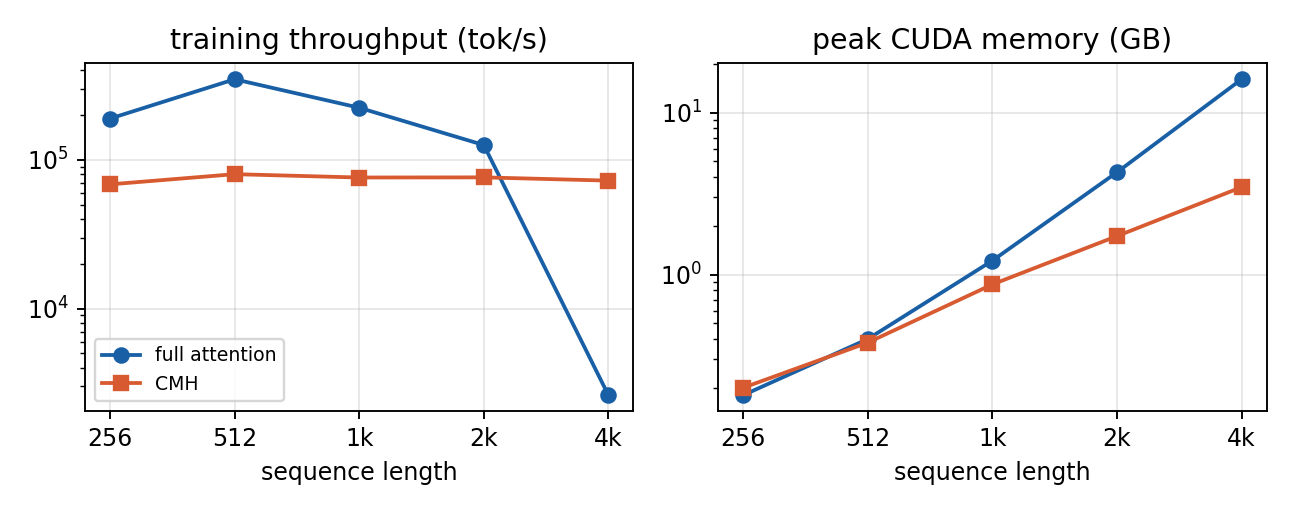
\includegraphics[width=0.95\textwidth]{fig_efficiency.png}
\caption{吞吐（左）与峰值 CUDA 显存（右）随序列长度的变化，双对数轴。全注意力成本上弯并在 4096 token 坍塌；\cmh{} 保持平坦。}
\label{fig:efficiency}
\end{figure}

\section{蒸馏实验：修复尝试及其失败}\label{sec:exp}

\subsection{设置}

\begin{table}[h]
\centering
\caption{训练配置。}
\label{tab:setup}
\begin{tabular}{ll}
\toprule
教师 & GPT-2（124M），冻结，bf16 前向 \\
学生 & \cmh{} 38.4M / full 33.7M / window 33.7M（8 层，$d{=}384$，$h{=}4$，$w{=}256$） \\
分词器 & GPT-2 BPE（50{,}257），嵌入--输出头权重绑定 \\
数据 & TinyStories \cite{eldan2023tinystories}，99M 训练 / 2M 验证 token，seq 512 \\
目标 & $\mathcal{L} = \alpha\,\mathrm{CE}(y, p_s) + (1-\alpha)\,T^2\,\mathrm{KL}(\sigma(z_t/T)\,\|\,\sigma(z_s/T))$ \\
蒸馏超参 & $T = 2$，$\alpha = 0.5$ \\
优化器 & AdamW，OneCycle LR $6{\times}10^{-4}$，6k 步（$\approx$74M token），batch 24 \\
\bottomrule
\end{tabular}
\end{table}

预期假设：蒸馏把"什么值得记"从发现问题转为监督回归问题——教师的 logits 在每个位置给出完整分布，应能为写入门控、保留率与状态内容提供稠密梯度通路，绕过 \S\ref{sec:scratch} 识别出的冷启动区域。\textbf{该假设被实验否定}（见下）。

\subsection{结果}

\begin{table}[h]
\centering
\caption{TinyStories 主结果（74M token 训练预算，所有学生的数据、分词器与调度完全一致）。}
\label{tab:main}
\begin{tabular}{lrr}
\toprule
模型 & 验证 CE & 困惑度 \\
\midrule
GPT-2 教师（124M，域外） & 2.4806 & 11.95 \\
\midrule
scratch-full（33.7M） & \textbf{1.7974} & \textbf{6.03} \\
scratch-window（33.7M） & \textbf{1.7945} & \textbf{6.02} \\
scratch-\cmh{}（38.4M） & 5.4435 & 231.25 \\
\midrule
distill-\cmh{} $\leftarrow$ GPT-2（38.4M） & 5.4010 & 221.63 \\
distill-\cmh{} $\leftarrow$ 域内全注意力教师（38.4M） & 5.5556 & 258.69 \\
\bottomrule
\end{tabular}
\end{table}

\begin{figure}[h]
\centering
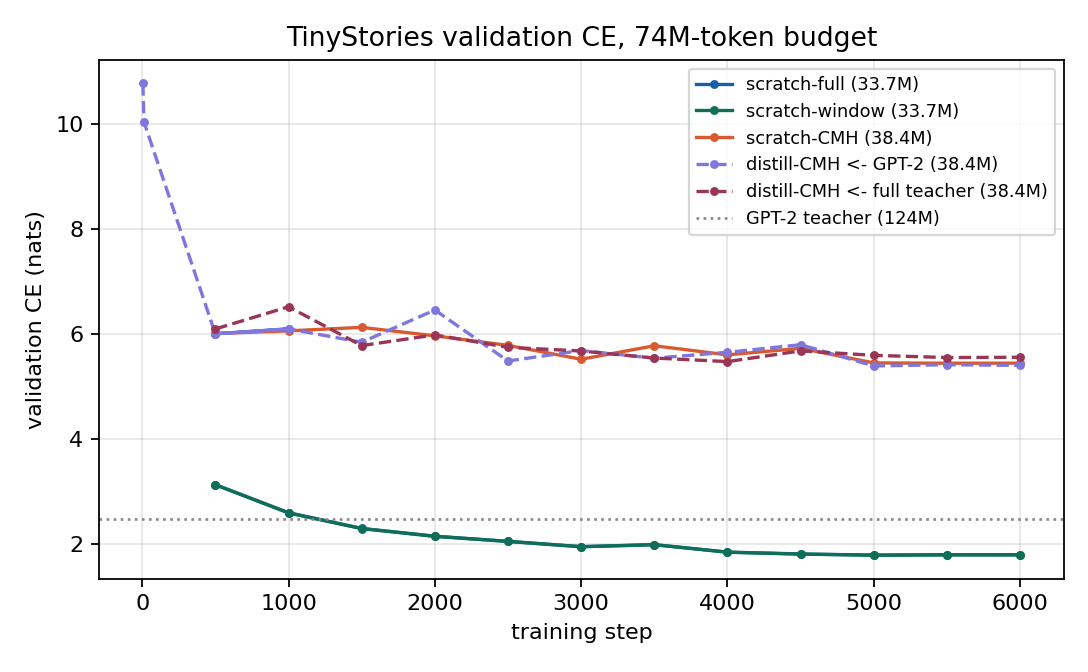
\includegraphics[width=0.85\textwidth]{val_curves.png}
\caption{训练全程的验证交叉熵。虚线为蒸馏学生；点线为域外 GPT-2 教师。纯滑窗与全注意力重合；两种 \cmh{} 蒸馏变体均停留在从零训练 \cmh{} 的平台上。}
\label{fig:curves}
\end{figure}

三个观察，均在完整训练过程中稳定成立：

\textbf{(1) 该语料几乎不需要全局上下文。}纯滑窗与全注意力仅差 0.003 nats（1.7945 对 1.7974）。全注意力在 256 token 跨度之外能提取的任何信息，这个数据集都不需要——因此 TinyStories 本身无法论证任何全局通道（记忆式的或其他）的价值。

\textbf{(2) 记忆通道在主动帮倒忙。}\cmh{} 得分 5.44，而其自身的纯滑窗消融为 1.79：门控联想读取（式~\ref{eq:read}）注入的残差净损失 3.65 nats，而非贡献信息。学生参数更多（38.4M 对 33.7M），本应在容量上占优；实际上软联想状态在此规模下是净负债。

\textbf{(3) 记忆通道不是死重——是拐杖。}推理时禁用联想读取与写入（窗口和 FFN 不变），\cmh{} 学生的验证 CE 从 5.41 升到 6.06：状态确实携带了约 0.65 nats 的真实信号，块也学会了依赖它。但正是这根拐杖让模型落后纯滑窗模型 3.6 nats——后者根本不需要拐杖。我们还检查了学到的保留率：所有层的所有头都停在 $\gamma = 0.924$，离 0.951 的初始化几乎没有移动，头与头之间没有特化——我们设计的"有的头记得更久"机制在可获得的训练信号下从未启用。

\textbf{(4) 蒸馏无法弥合差距——弱教师和强教师都不行。}来自 GPT-2 的 KD 带来 $-0.04$ nats；来自域内教师（2.48，在本文语料上比 GPT-2 好 0.7 nats）的 KD 带来 $+0.11$。决定性的观察是：两个蒸馏学生都\textbf{比自己教师差 2.9--3.1 nats}——学生连被监督的目标分布本身都拟合不进去，因此瓶颈是\textbf{表示能力}（固定状态读取），而非监督信号。\S\ref{sec:scratch} 的冷启动假说由此得到强化并变得更加精确：稠密的逐位置监督是\textbf{必要但非充分}条件；架构必须能够表示教师的寻址行为，蒸馏才可能把它转移过来。

\section{讨论与局限}\label{sec:discussion}

\textbf{负结果确立了什么。}冷启动分析为一条经验定理提供了架构层面的证据，并划出了精确边界：固定软联想状态既无法从稀疏任务信号、\textbf{也无法从稠密的教师监督}中习得精确检索。蒸馏的预言被直接检验并失败——这把责任从训练信号转移到归一化外积读取的\textbf{表示能力}上。

\textbf{局限。}(i) 全部实验在 $\le$40M 参数规模，失败与修复的规模行为均未验证。(ii) 评测语料为英文儿童故事；检索密集基准（Long Range Arena、大海捞针）留待后续。(iii) 学生全局通道的读写参数跨位置共享，位置寻址完全依赖可学习位置嵌入，无法外推到训练长度之外。(iv) 记忆读取是软凸组合；硬检索（离散寻址）是开放方向。

\textbf{未来工作。}(1) delta-rule 写入 \cite{yang2023delta}——允许写入键覆写自身绑定，已知能锐化检索；(2) 混合方案：蒸馏 + 少量全注意力层，对齐工业实践；(3) 规模化研究——记忆通道的优势是否随规模涌现。

\section{结论}

\cmh{} 证明了"用固定状态换 $O(N^2)$"的取舍恰好在效率维度兑现：吞吐至 4096 token 保持平坦（4096 处为全注意力的 15.2 倍）、显存节省 78\%。但在质量维度它决定性地失败：门控联想记忆通道在真实语言上比其自身的纯滑窗消融\textbf{净损失 3.65 nats}，且无论从零训练还是 token 级蒸馏——弱教师或强教师——都无法弥合这一差距的任何部分。在语料几乎不需要全局上下文的序列长度下，纯滑窗即可匹敌全注意力；在需要更多时，我们的证据表明固定软联想状态在此规模下无法提供。保留显式全注意力层的混合设计因此得到实证支持，而这一方向的进展很可能需要\textbf{架构上不同的全局通道}（delta-rule 写入、硬寻址、可学习槽键），而非更好的训练信号。

\section*{致谢}

代码、实验执行与初稿撰写使用了 AI 编程辅助。全部实验结果由随文公开的脚本产出，并与训练日志逐一核对；作者核查了每一条引用、图例与论断，并对全文内容负全责。代码、训练日志与故事接龙演示：\url{https://github.com/mierstan/CMH}。

\bibliographystyle{plain}
\begin{thebibliography}{20}

\bibitem{vaswani2017} A.~Vaswani et al.
\newblock Attention is all you need.
\newblock \emph{NeurIPS}, 2017.

\bibitem{katharopoulos2020} A.~Katharopoulos, A.~Vyas, N.~Pappas, F.~Fleuret.
\newblock Transformers are RNNs: Fast autoregressive transformers with linear attention.
\newblock \emph{ICML}, 2020.

\bibitem{gu2023mamba} A.~Gu, T.~Dao.
\newblock Mamba: Linear-time sequence modeling with selective state spaces.
\newblock \emph{arXiv:2312.00752}, 2023.

\bibitem{peng2023rwkv} B.~Peng et al.
\newblock RWKV: Reinventing RNNs for the transformer era.
\newblock \emph{EMNLP}, 2023.

\bibitem{yang2023gla} S.~Yang, B.~Wang, Y.~Zhang, Y.~Shen, D.~Schuurmans.
\newblock Gated linear attention transformers with hardware-efficient training.
\newblock \emph{arXiv:2312.06635}, 2023.

\bibitem{sun2023retnet} Y.~Sun et al.
\newblock Retentive network: A successor of transformer for large language models.
\newblock \emph{arXiv:2307.08621}, 2023.

\bibitem{yang2023delta} S.~Yang et al.
\newblock Parallelizing linear transformers with the delta rule over sequence length.
\newblock \emph{arXiv:2406.06484}, 2024.

\bibitem{beltagy2020longformer} I.~Beltagy, M.~E.~Peters, A.~Cohan.
\newblock Longformer: The long-document transformer.
\newblock \emph{arXiv:2004.05168}, 2020.

\bibitem{waleffe2024jamba} R.~Waleffe et al.
\newblock Jamba: A hybrid transformer-Mamba language model.
\newblock \emph{arXiv:2403.19887}, 2024.

\bibitem{glorioso2024zamba} P.~Glorioso et al.
\newblock Zamba: A compact 7B state-space hybrid model.
\newblock \emph{arXiv:2405.16712}, 2024.

\bibitem{wang2024samba} J.~Wang et al.
\newblock Samba: Simple hybrid state space models for efficient unlimited context language modeling.
\newblock \emph{arXiv:2406.07522}, 2024.

\bibitem{wang2024hymba} X.~Wang et al.
\newblock Hymba: A hybrid-head architecture for small language models.
\newblock \emph{arXiv:2411.13676}, 2024.

\bibitem{wang2024mohawk} Y.~Wang et al.
\newblock MOHAWK: Mamba distilled in the trenches of long context.
\newblock \emph{arXiv:2408.00140}, 2024.

\bibitem{wang2024mambaillama} J.~Wang et al.
\newblock Mamba in the Llama: Distilling and accelerating hybrid models.
\newblock \emph{arXiv:2408.04029}, 2024.

\bibitem{hinton2015distill} G.~Hinton, O.~Vinyals, J.~Dean.
\newblock Distilling the knowledge in a neural network.
\newblock \emph{arXiv:1503.02531}, 2015.

\bibitem{eldan2023tinystories} R.~Eldan, Y.~Li.
\newblock TinyStories: How small can language models be and still speak coherent English?
\newblock \emph{arXiv:2305.07759}, 2023.

\end{thebibliography}

\end{document}
